\part{Práctica 2}
\section{Actividad 2-1}
\label{p21}
\begin{center}
    \parbox{12cm}{\justify\textit{Para esta práctica, utilice el conjunto de datos de altura de ola proporcionado en Moodle.\\
    Describa las operaciones de preprocesamiento que ha realizado sobre la base de datos proporcionada y cómo queda la base de datos final ya preprocesada. Se deja a su elección el conjunto de técnicas a aplicar, así como el nivel de detalle y descripción que quiera dar a su trabajo. \\   
    Para probar rendimientos sobre su preprocesamiento, puede lanzar cualquier algoritmo de Weka, por ejemplo classifiers.functions.Logistic, y fijarse en la métrica ``Correctly Classified Instances''. En la opción ``Suplied test set'' se indicaría el fichero del conjunto de test, mientras que el de entrenamiento corresponde al que se ha cargado desde la pestaña Preprocess.}}
\end{center}

\subsection{Introducción}
En este ejercicio se van a poner en práctica los conceptos aprendidos sobre preprocesamiento de datos. Para ello se utilizará una base de datos de observaciones meteorológicas tomadas entre 2014 y 2016 a razón de 4 mediciones al día. El conjunto tiene 3559 patrones con 17 atributos numéricos y una clase nominal. Los atributos son:
\begin{itemize}
    \item AIR: Temperatura del aire en la superficie (ºK).
    \item PRES: Presión a nivel de superficie (Pa).
    \item RHUM: Humedad relativa a nivel de superficie (\%).
    \item UWND: Velocidad del viento de oeste a este (eje X) (m/s).
    \item VWND: Velocidad del viento de sur a norte (eje Y) (m/s).
    \item WDIR: Dirección del viento en el sentido de las agujas del reloj (grad).
    \item WSPD: Velocidad del viento (m/s).
    \item GST: Velocidad de pico del viento (m/s).
    \item DPD: Periodo de ola dominante (s).
    \item APD: Periodo medio de ol a dominante (s).
    \item MWD: Dirección de la que viene el periodo de ola dominante (grad).
    \item PRES: Presión a nivel de superficie (HPa).
    \item ATMP: Temperatura del aire en la parte superior de la boya (ºC).
    \item WTMP: Temperatura a nivel del mar (ºC).
    \item DEWP: Punto de rocío tomado a la misma altura que ATMP (ºC).
    \item VIS: Visibilidad desde la boya (MN).
    \item TIDE: NIvel del agua por encima o por debajo de la media inferior del agua (Pies).
\end{itemize}
La variable de salida indica la altura de ola en las seis horas siguientes. Es discreta con valores Baja, Media, Moderada y MuyAlta.

Para valorar el preprocesamiento realizado, se generará a cada paso un clasificador logístico y se evaluará con un conjunto de pruebas con la misma estructura que contiene los datos correspondientes a los años 2017 y 2018. Este proceso se realiza desde la pestaña Classify de Weka Explorer. El clasificador seleccionado será Functions.Logistic con la configuración indicada en la figura \ref{fig:classifiers-functions-logistic-config} y utilizando como conjunto de test el archivo \code{alturaolatest.arff}, al que previamente se le habrá realizado el correspondiente tratamiento.

\begin{figure}[ht]
    \centering
    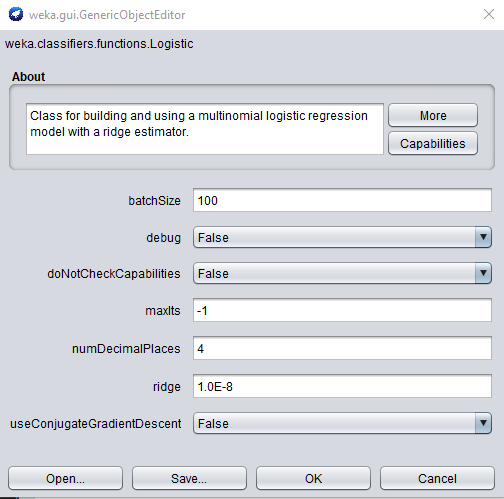
\includegraphics[scale=0.4]{classifiers-functions-logistic-config}
    \caption{Configuración del clasificador logístico}
    \label{fig:classifiers-functions-logistic-config}
\end{figure}

\subsection{Preparación}
Como paso previo se han convertido los archivos \code{.csv} a \code{.arff}. Los dos archivos se han cargado en Weka para poder visualizar su contenido, como puede verse en las figuras \ref{fig:altura-ola-orig} y \ref{fig:altura-ola-test-orig}.

\begin{figure}[H]
    \centering
    \begin{minipage}{0.5\textwidth}
        \centering
        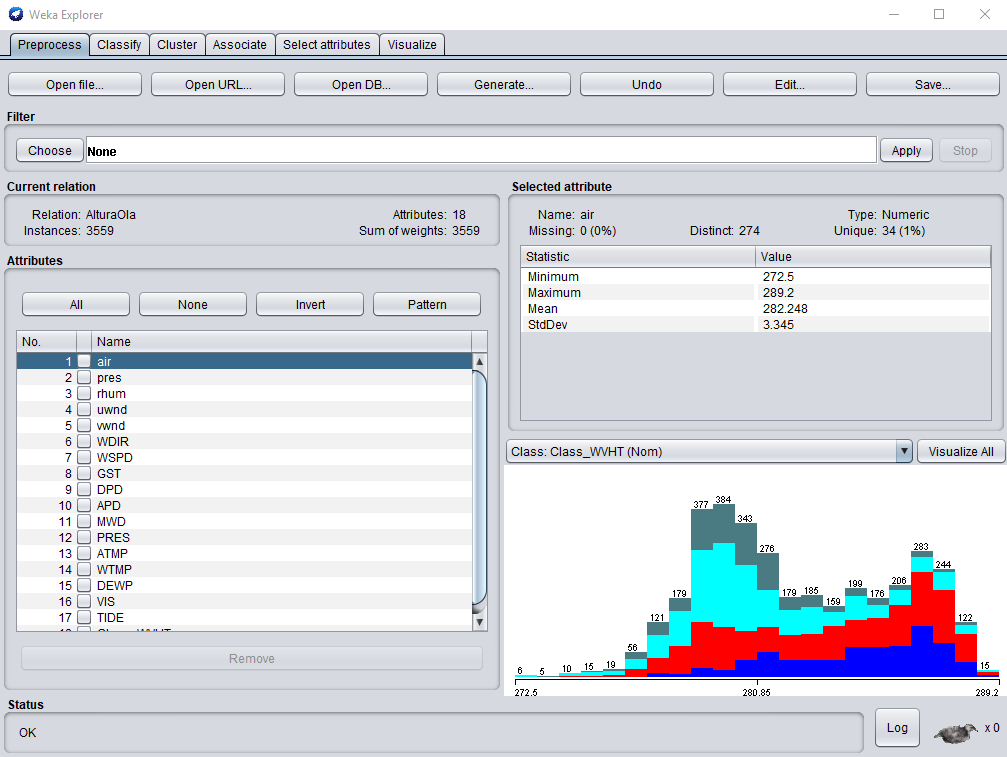
\includegraphics[scale=0.29]{altura-ola-orig}
        \caption{Captura de \code{alturaola.arff}.}
        \label{fig:altura-ola-orig}
    \end{minipage}\hfill
    \begin{minipage}{0.5\textwidth}
        \centering
        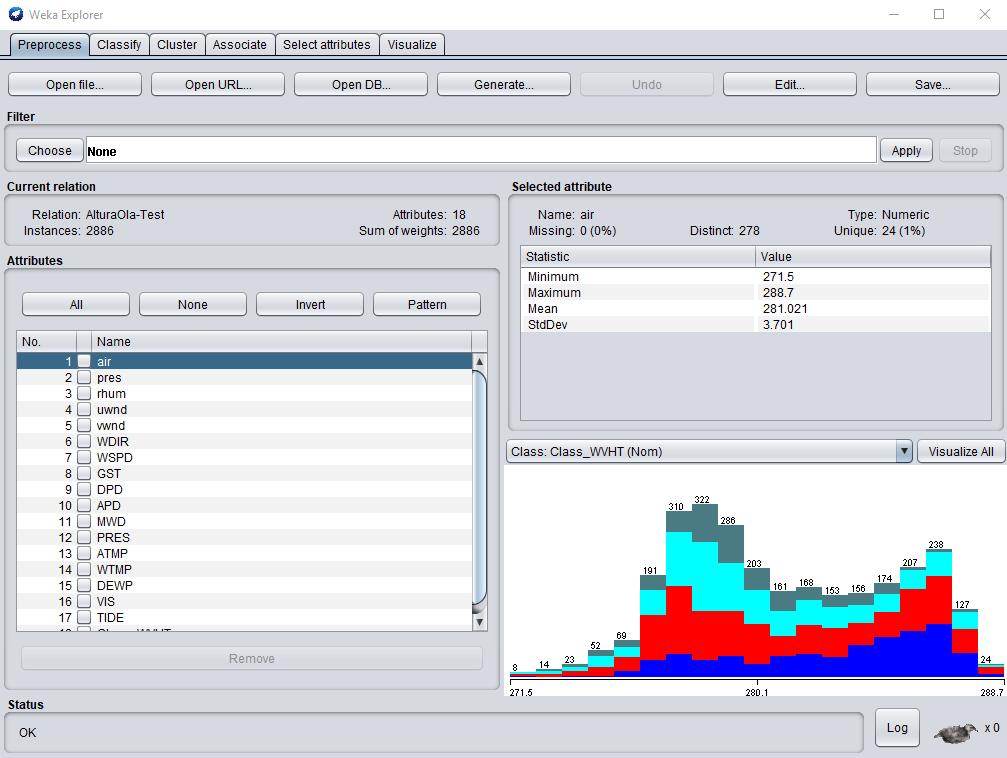
\includegraphics[scale=0.29]{altura-ola-test-orig}
        \caption{Captura de \code{alturaolatest.arff}.}
        \label{fig:altura-ola-test-orig}
    \end{minipage}
\end{figure}

Tras la conversión de los archivos y antes de empezar el tratamiento de los datos, se ha generado y testeado el clasificador logístico para ver el punto de partida. En la figura \ref{fig:clasificador-logistico-resultados-00} se pueden observar los resultados: se tiene en el punto de partida un $71.9335\%$ de patrones correctamente clasificados y precisión mínima de $0.660$ para la clase ``Media''.

\begin{figure}[ht]
    \centering
    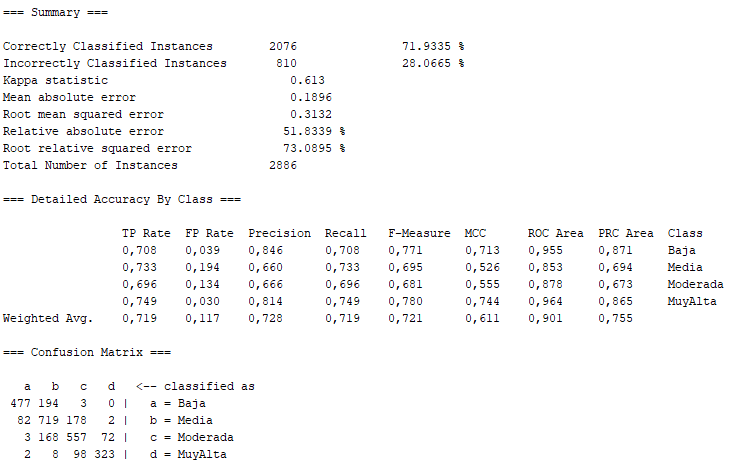
\includegraphics[scale=0.8]{clasificador-logistico-resultados-00}
    \caption{Resultados del clasificador logístico antes del tratamiento de datos.}
    \label{fig:clasificador-logistico-resultados-00}
\end{figure}

\subsection{Datos perdidos}
En primer lugar se eliminan los tres atributos con 100\% de datos perdidos: TIDS, VIS y MWD tanto en el conjunto de entrenamiento como en el de test y se genera de nuevo el clasificador logístico. Como se puede observar en la figura \ref{fig:clasificador-logistico-resultados-01}, la eliminación de los atributos con 100\% de datos perdidos no tiene ningún efecto.

\begin{figure}[ht]
    \centering
    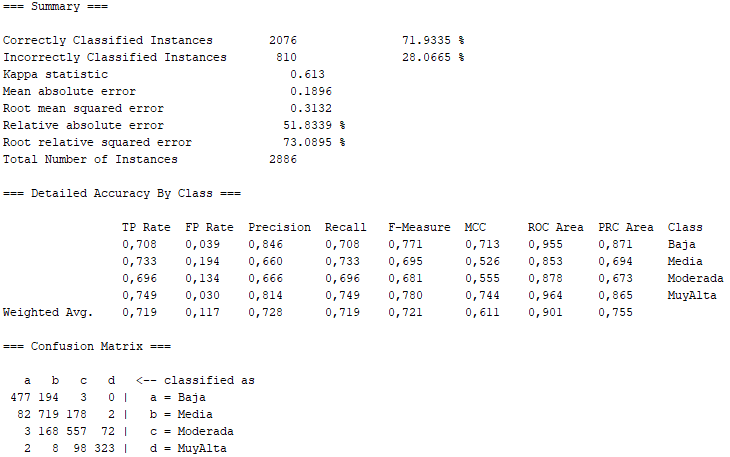
\includegraphics[trim={0cm 10.4cm 7cm 0.7cm},clip]{clasificador-logistico-resultados-01}
    \caption{Resultados tras eliminar TIDS, VIS y MWD.}
    \label{fig:clasificador-logistico-resultados-01}
\end{figure}
% Datos en alturaola.02.datos-perdidos-a.arff y alturaolatest.02-datos-perdidos-a.arff

A continuación se estudian los campos con valores perdidos que son en entrenamiento DPD, APD, PRES y DEWP con 8 (<1\%), 8 (<1\%), 553 (16\%) y 1189 (33\%) patrones con datos perdidos respectivamente y en pruebas WSPD, GST, DPD, APD, PRES, ATMP, WTMP Y DEWP. Para estos casos se reemplazan los valores perdidos por la media de la clase calculada sobre el conjunto de entrenamiento tanto en el conjunto de entrenamiento como en el conjunto de generalización (ver cuadro \ref{tab:medias-por-clase}). Se realiza este procedimiento siguiendo el consejo del archivo \code{Imputación de valores perdidos mas justa en training y test.pdf}, aunque me preocupa en qué medida contribuirá al rendimiento del modelo cuando se exponga a datos nuevos.

\begin{table}[ht]
    \centering
    \begin{tabular}{|r|rlrl|rrrr|}
    \hline
      \multicolumn{1}{|c|}{} &
      \multicolumn{4}{c|}{Datos perdidos} &
      \multicolumn{4}{c|}{Medias en entrenamiento} \\
      \multicolumn{1}{|c|}{Atributo} &
      \multicolumn{2}{c}{Entrenamiento} &
      \multicolumn{2}{c|}{Test} &
      \multicolumn{1}{c}{Baja} &
      \multicolumn{1}{c}{Media} &
      \multicolumn{1}{c}{Moderada} &
      \multicolumn{1}{c|}{MuyAlta} \\ \hline
      WSPD & 0    & (0\%)  & 1    & (<1\%)  & 4,6    & 6,6    & 8,4    & 11,9   \\ 
      GST  & 0    & (0\%)  & 9    & (<1\%)  & 5,6    & 8,1    & 10,5   & 14,9   \\
      DPD  & 8    & (<1\%) & 21   & (1\%)   & 11,5   & 10,3   & 10,8   & 11,7   \\
      APD  & 8    & (<1\%) & 21   & (1\%)   & 6,5    & 6,7    & 7,0    & 7,7    \\
      PRES & 553  & (16\%) & 6    & (<1\%)  & 1017,8 & 1013,1 & 1008,7 & 1007,2 \\
      ATMP & 0    & (0\%)  & 3    & (<1\%)  & 11,5   & 9,9    & 7,8    & 7,4    \\
      WTMP & 0    & (0\%)  & 7    & (<1\%)  & 12,3   & 10,8   & 8,8    & 8,2    \\
      DEWP & 1189 & (33\%) & 2886 & (100\%) & 8,9    & 7,1    & 4,8    & 4,8    \\\hline
    \end{tabular}
    \caption{Datos perdidos y medias de atributos en entrenamiento por clase.}
    \label{tab:medias-por-clase}
\end{table}

Una vez reemplazados todos los datos perdidos se obtienen en el clasificador los resultados mostrados en la figura \ref{fig:clasificador-logistico-resultados-02b}, en los que se observa una mejora en las métricas del clasificador. Por ejemplo, el CCR sube casi un 3\%, la mínima sensibilidad aumenta ligeramente y el área bajo la curva ROC aumenta para tres de las cuatro clases.
% Datos en alturaola.02.datos-perdidos-b.arff y alturaolatest.02-datos-perdidos-b.arff

\begin{figure}[ht]
    \centering
    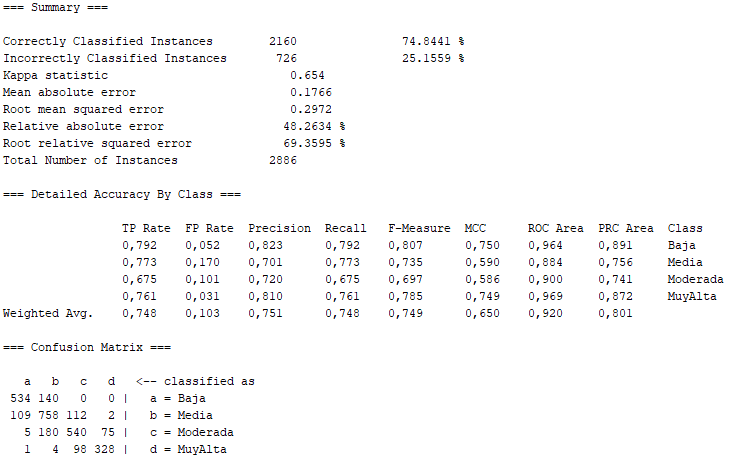
\includegraphics[scale=0.8]{clasificador-logistico-resultados-02}
    \caption{Resultados tras reemplazar los datos perdidos}
    \label{fig:clasificador-logistico-resultados-02b}
\end{figure}

\subsection{Unificación de medidas}
El siguiente paso a seguir será la estandarización de las unidades de medida de los atributos que representan la misma magnitud. En nuestro dataset tenemos dos pares de atributos que representan temperatura y presión respectivamente, y utilizan diferentes unidades (ºC/ºK por un lado y HPas/Pas), por lo que correspondería a unificarlas. Las transformaciones se han realizado mediante el filtro \code{MathExpression}. Primero se han pasado a Pascales los valores del atributo PRES que estaban en HPas y seguidamente se han pasado a ºC los valores del atributo \code{air} que se encontraban en ºK. Como era de esperar, estas operaciones no han tenido ningún efecto sobre el resultado del clasificador.
% Datos en alturaola.03.unidades.arff y alturaolatest.03.unidades.arff

\subsection{Selección de características}
En esta etapa del preprocesamiento vamos a intentar detectar los atributos que influyen muy poco en la clase (atributos irrelevantes) para así eliminarlos y simplificar el modelo. Del mismo modo, intentaremos identificar pares de atributos con una correlación alta (atributos redundantes) para prescindir, de entre los dos, de el que menos influya en la clase.

\subsubsection{Análisis de atributos irrelevantes}
Para medir la influencia de cada atributo sobre la clase del dataset en Weka utilizaremos el evaluador de atributos \code{CorrelationAttributeEval} en combinación con \code{Ranker} como método de búsqueda en la pestaña ``Select attributes'' del explorador de Weka. La salida de este análisis se puede ver en la figura \ref{fig:correlation-attribute-eval}.

\begin{figure}[H]
    \centering
    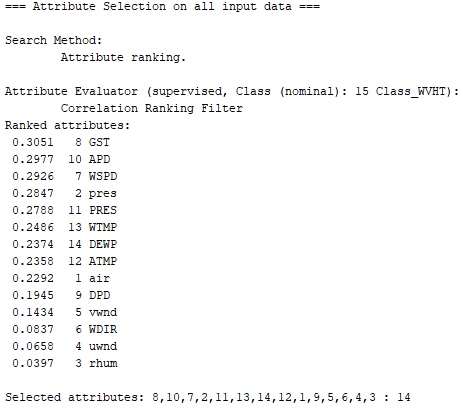
\includegraphics[scale=0.51]{03-correlation-attribute-eval}
    \caption{Resultados de \code{CorrelationAttributeEval}}
    \label{fig:correlation-attribute-eval}
\end{figure}

Lo siguiente será eliminar uno por uno atributos desde el menos influyente (\code{rhum}) hacia arriba comprobando el resultado del clasificador logístico hasta que comience a empeorar. Se eliminan \code{rhum} y \code{uwnd} para alcanzar un $CCR=75,23\%$ (fig. \ref{fig:03-quitar-irrelevantes}), pero al eliminar \code{WDIR} vemos que empeora, por lo que paramos ahí. No estoy seguro de si este paso para reducir la complejidad conviene o no conviene en este caso ya que a pesar de la leve mejora del CCR, vemos en la matriz de confusión que la única clase que ha mejorado en nº de patrones bien clasificados es \code{Media}, que ya era la que mejor clasificaba, a costa de un empeoramiento en el resto. 

\begin{figure}[ht]
    \centering
    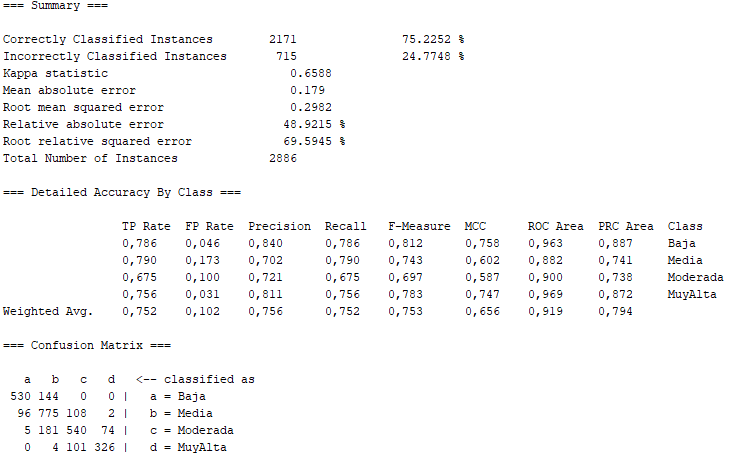
\includegraphics[scale=0.8]{03-quitar-irrelevantes}
    \caption{Resultados tras eliminar atributos irrelevantes}
    \label{fig:03-quitar-irrelevantes}
\end{figure}


\subsubsection{Análisis de atributos redundantes}
A continuación se estudiará la correlación entre atributos. Para realizar este análisis en Weka utilizamos el evaluador de atributos \code{PrincipalComponents} junto con el buscador \code{Ranker}. Podemos ver la tabla de correlaciones obtenida en el cuadro \ref{cuadro:correlaciones}, en el que se han marcado en rojo, naranja y amarillo las correlaciones por encima de 0,6 según su importancia (rojo la más importante). El proceso de eliminación de atributos correlados será el siguiente:
\begin{enumerate}
    \item Elegir un par atributos con correlación alta.
    \item Del par elegido, eliminar el atributo menos correlado con la clase según la figura \ref{fig:correlation-attribute-eval}.
    \item Generar y evaluar el clasificador logístico.
    \begin{enumerate}
        \item Si el resultado mejora, se mantiene la eliminación del atributo.
        \item Si no mejora, se restituye el atributo.
    \end{enumerate}
\end{enumerate}

\begin{table}[]
    \resizebox{\textwidth}{!}{%
    \begin{tabular}{|
    >{\columncolor[HTML]{9B9B9B}}c |rrrrrrrrrrrr|}
    \hline
    \cellcolor[HTML]{FFFFFF}{\color[HTML]{FFFFFF} } & \multicolumn{1}{c}{\cellcolor[HTML]{9B9B9B}{\color[HTML]{FFFFFF} air}} & \multicolumn{1}{c}{\cellcolor[HTML]{9B9B9B}{\color[HTML]{FFFFFF} pres}} & \multicolumn{1}{c}{\cellcolor[HTML]{9B9B9B}{\color[HTML]{FFFFFF} vwnd}} & \multicolumn{1}{c}{\cellcolor[HTML]{9B9B9B}{\color[HTML]{FFFFFF} WDIR}} & \multicolumn{1}{c}{\cellcolor[HTML]{9B9B9B}{\color[HTML]{FFFFFF} WSPD}} & \multicolumn{1}{c}{\cellcolor[HTML]{9B9B9B}{\color[HTML]{FFFFFF} GST}} & \multicolumn{1}{c}{\cellcolor[HTML]{9B9B9B}{\color[HTML]{FFFFFF} DPD}} & \multicolumn{1}{c}{\cellcolor[HTML]{9B9B9B}{\color[HTML]{FFFFFF} APD}} & \multicolumn{1}{c}{\cellcolor[HTML]{9B9B9B}{\color[HTML]{FFFFFF} PRES}} & \multicolumn{1}{c}{\cellcolor[HTML]{9B9B9B}{\color[HTML]{FFFFFF} ATMP}} & \multicolumn{1}{c}{\cellcolor[HTML]{9B9B9B}{\color[HTML]{FFFFFF} WTMP}} & \multicolumn{1}{c|}{\cellcolor[HTML]{9B9B9B}{\color[HTML]{FFFFFF} DEWP}} \\ \hline
    {\color[HTML]{FFFFFF} air} & \cellcolor[HTML]{9B9B9B}{\color[HTML]{FFFFFF} 1} & 0,23 & -0 & 0,1 & -0,15 & -0,18 & -0,34 & -0,44 & 0,23 & \cellcolor[HTML]{FE0000}{\color[HTML]{FFFFFF} 0,98} & \cellcolor[HTML]{FE0000}{\color[HTML]{FFFFFF} 0,94} & \cellcolor[HTML]{F8A102}{\color[HTML]{FFFFFF} 0,77} \\
    {\color[HTML]{FFFFFF} pres} & 0,23 & \cellcolor[HTML]{9B9B9B}{\color[HTML]{FFFFFF} 1} & -0,2 & 0,25 & -0,34 & -0,37 & -0,26 & -0,43 & \cellcolor[HTML]{FE0000}{\color[HTML]{FFFFFF} 0,95} & 0,26 & 0,26 & 0,22 \\
    {\color[HTML]{FFFFFF} vwnd} & -0 & -0,2 & \cellcolor[HTML]{9B9B9B}{\color[HTML]{FFFFFF} 1} & -0,15 & 0,31 & 0,31 & 0,07 & 0,13 & -0,2 & -0,01 & -0,12 & 0,08 \\
    {\color[HTML]{FFFFFF} WDIR} & 0,1 & 0,25 & -0,15 & \cellcolor[HTML]{9B9B9B}{\color[HTML]{FFFFFF} 1} & -0,06 & -0,07 & -0,04 & -0,09 & 0,17 & 0,14 & 0,2 & 0,05 \\
    {\color[HTML]{FFFFFF} WSPD} & -0,15 & -0,34 & 0,31 & -0,06 & \cellcolor[HTML]{9B9B9B}{\color[HTML]{FFFFFF} 1} & \cellcolor[HTML]{FE0000}{\color[HTML]{FFFFFF} 0,99} & 0,02 & 0,1 & -0,34 & -0,17 & -0,21 & -0,18 \\
    {\color[HTML]{FFFFFF} GST} & -0,18 & -0,37 & 0,31 & -0,07 & \cellcolor[HTML]{FE0000}{\color[HTML]{FFFFFF} 0,99} & \cellcolor[HTML]{9B9B9B}{\color[HTML]{FFFFFF} 1} & 0,04 & 0,14 & -0,36 & -0,2 & -0,23 & -0,21 \\
    {\color[HTML]{FFFFFF} DPD} & -0,34 & -0,26 & 0,07 & -0,04 & 0,02 & 0,04 & \cellcolor[HTML]{9B9B9B}{\color[HTML]{FFFFFF} 1} & \cellcolor[HTML]{F8A102}{\color[HTML]{FFFFFF} 0,71} & -0,27 & -0,33 & -0,31 & -0,3 \\
    {\color[HTML]{FFFFFF} APD} & -0,44 & -0,43 & 0,13 & -0,09 & 0,1 & 0,14 & \cellcolor[HTML]{F8A102}{\color[HTML]{FFFFFF} 0,71} & \cellcolor[HTML]{9B9B9B}{\color[HTML]{FFFFFF} 1} & -0,45 & -0,44 & -0,44 & -0,41 \\
    {\color[HTML]{FFFFFF} PRES} & 0,23 & \cellcolor[HTML]{FE0000}{\color[HTML]{FFFFFF} 0,95} & -0,2 & 0,17 & -0,34 & -0,36 & -0,27 & -0,45 & \cellcolor[HTML]{9B9B9B}{\color[HTML]{FFFFFF} 1} & 0,24 & 0,25 & 0,2 \\
    {\color[HTML]{FFFFFF} ATMP} & \cellcolor[HTML]{FE0000}{\color[HTML]{FFFFFF} 0,98} & 0,26 & -0,01 & 0,14 & -0,17 & -0,2 & -0,33 & -0,44 & 0,24 & \cellcolor[HTML]{9B9B9B}{\color[HTML]{FFFFFF} 1} & \cellcolor[HTML]{FE0000}{\color[HTML]{FFFFFF} 0,95} & \cellcolor[HTML]{F8A102}{\color[HTML]{FFFFFF} 0,76} \\
    {\color[HTML]{FFFFFF} WTMP} & \cellcolor[HTML]{FE0000}{\color[HTML]{FFFFFF} 0,94} & 0,26 & -0,12 & 0,2 & -0,21 & -0,23 & -0,31 & -0,44 & 0,25 & \cellcolor[HTML]{FE0000}{\color[HTML]{FFFFFF} 0,95} & \cellcolor[HTML]{9B9B9B}{\color[HTML]{FFFFFF} 1} & \cellcolor[HTML]{FFC702}0,66 \\
    {\color[HTML]{FFFFFF} DEWP} & \cellcolor[HTML]{F8A102}{\color[HTML]{FFFFFF} 0,77} & 0,22 & 0,08 & 0,05 & -0,18 & -0,21 & -0,3 & -0,41 & 0,2 & \cellcolor[HTML]{F8A102}{\color[HTML]{FFFFFF} 0,76} & \cellcolor[HTML]{FFC702}0,66 & \cellcolor[HTML]{9B9B9B}{\color[HTML]{FFFFFF} 1} \\ \hline
    \end{tabular}%
    }
    \caption{Correlaciones entre atributos}
    \label{cuadro:correlaciones}
\end{table}
El primer par procesado ha sido \code{pres-PRES} porque tiene una altísima correlación y no es de los atributos más influyentes sobre la clase, pero principalmente porque representan la misma magnitud. Tras la eliminación de \code{PRES}, el clasificador apenas cambia. Sólo mejora muy ligeramente, lo que nos da una idea de lo poco que servía el atributo eliminado, ganando el modelo en simplicidad.

El segundo par procesado ha sido \code{WSPD-GST} por tener la más alta correlación. De los dos atributos, se ha eliminado WSPD por ser el que menos influye sobre la clase. Tras la eliminación, el clasificador apenas ha cambiado. Sólo 8 patrones correctamente clasificados menos, lo que nos lleva a un CCR de $75,09\%$ con una sensibilidad mínima de $0,679$ para la clase <<Moderada>>.

La siguiente correlación más alta se da entre el par \code{air-ATMP}. \code{air} está fuertemente correlacionado con \code{WTMP} y \code{DEWP} también, y al mismo tiempo es el menos correlacionado con la clase de los cuatro, por lo que se va a eliminar. Tras la eliminación vemos que los estadísticos se ven muy poco afectados: $CCR=75,05\%$ y sensibilidad mínima de $0,686$ para la clase <<Moderada>>.

El par \code{WTMP-ATMP} es el siguiente más correlacionado. Como \code{ATMP} es el atributo que menos influye sobre la clase, se elimina éste. El clasificador empeora significativamente pasando a un $CCR=74,22\%$ por lo que se decide no mantener esta eliminación. La eliminación de \code{WTMP} produce un efecto similar ($CCR=74,64\%$), por lo tanto se mantendrán estos dos atributos.

El siguiente par estudiado ha sido \code{APD-DPD}, ya con correlación más baja. El atributo \code{DPD} es mucho menos influyente en la clase, por lo que se decide eliminarlo consiguiendo un ligero aumento de rendimiento en el porcentaje de patrones bien clasificados ($CCR=75,16\%$) así como en la sensibilidad mínima ($0,690$).

El último par es \code{DEWP-WTMP}. \code{DEWP} influye menos en la clase y además, ya se comprobó la influencia negativa de la eliminación de \code{WTMP} en el rendimiento del clasificador, por lo que se elimina \code{DEWP}. Esta eliminación ha tenido un impacto muy negativo sobre el clasificador $CCR=71,86\%$. Por este motivo, la eliminación se revierte y no se eliminan más atributos.

En resumen, se han eliminado los atributos \code{pres}, \code{WSPD}, \code{air} y \code{DPD} reduciendo la complejidad del modelo. Al mismo tiempo, los indicadores del modelo como CCR y mínima sensibilidad han mejorado, alcanzando valores $75,16\%$ y $0,690$ respectivamente (ver figura \ref{fig:clasificador-logistico-resultados-04}).

\begin{figure}[ht]
    \centering
    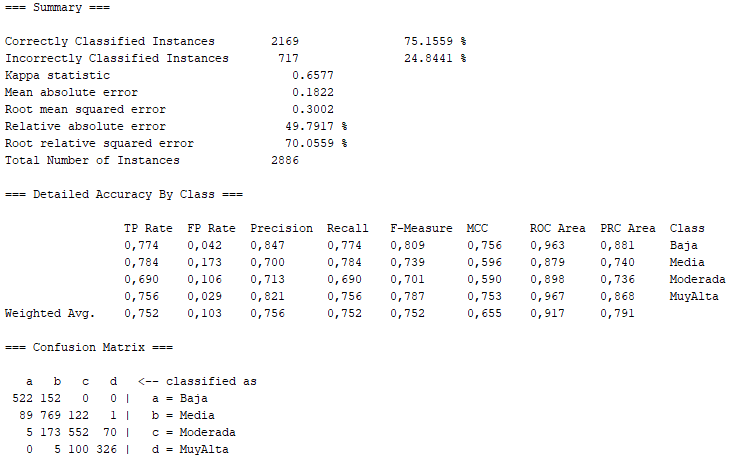
\includegraphics[scale=0.8]{clasificador-logistico-resultados-04}
    \caption{Resultados tras quitar atributos redundantes}
    \label{fig:clasificador-logistico-resultados-04}
\end{figure}


\subsection{Normalización}
El siguiente paso del preprocesamiento consiste en normalizar los datos tanto de entrenamiento como de generalización. Queremos llevar cada atributo a un rango $[0-1]$ en entrenamiento y luego aplicar la misma transformación al conjunto de generalización. Para ello, aplicaremos la fórmula \ref{formula:normalizacion} a cada atributo de ambos conjuntos pero utilizando siempre los máximos y mínimos del conjunto de entrenamiento, tal como aparecen en la tabla \ref{cuadro:maximos-minimos-normalizacion}. El proceso se realizará mediante el filtro \code{MathExpression}, campo a campo. Para el conjunto de entrenamiento se obtiene el mismo resultado utilizando el filtro \code{Normalize}.
\begin{equation} \label{formula:normalizacion}
    a^*=\frac{a-a_{min}}{a_{max}-a_{min}}
\end{equation}

\begin{table}[ht]
    \centering
    \begin{tabular}{|r|r|r|r|r|r|r|r|}
    \hline
    \rowcolor[HTML]{9B9B9B} 
    {\color[HTML]{FFFFFF} } & \multicolumn{1}{c|}{\cellcolor[HTML]{9B9B9B}{\color[HTML]{FFFFFF} pres}} & \multicolumn{1}{c|}{\cellcolor[HTML]{9B9B9B}{\color[HTML]{FFFFFF} vwnd}} & \multicolumn{1}{c|}{\cellcolor[HTML]{9B9B9B}{\color[HTML]{FFFFFF} WDIR}} & \multicolumn{1}{c|}{\cellcolor[HTML]{9B9B9B}{\color[HTML]{FFFFFF} GST}} & \multicolumn{1}{c|}{\cellcolor[HTML]{9B9B9B}{\color[HTML]{FFFFFF} APD}} & \multicolumn{1}{c|}{\cellcolor[HTML]{9B9B9B}{\color[HTML]{FFFFFF} ATMP}} & \multicolumn{1}{c|}{\cellcolor[HTML]{9B9B9B}{\color[HTML]{FFFFFF} WTMP}} \\ \hline
    \cellcolor[HTML]{9B9B9B}{\color[HTML]{FFFFFF} min} & 96020 & -17,9 & 0 & 0,4 & 3,10 & -0,9 & 6 \\ \cline{1-1}
    \cellcolor[HTML]{9B9B9B}{\color[HTML]{FFFFFF} max} & 103850 & 21,1 & 359 & 26,1 & 11,09 & 15,8 & 16,1 \\ \cline{1-1}
    \cellcolor[HTML]{9B9B9B}{\color[HTML]{FFFFFF} ran} & 7830 & 39,0 & 359 & 25,7 & 7,99 & 16,7 & 10,1 \\ \hline
    \end{tabular}
    \caption{}
    \label{cuadro:maximos-minimos-normalizacion}
\end{table}

Como se puede comprobar en la figura \ref{fig:clasificador-logistico-resultados-05}, el proceso de normalización ha provocado un empeoramiento generalizado del rendimiento del clasificador, con casi un 4\% menos de patrones correctamente clasificados. No tengo claro que necesariamente cualquier clasificador deba ser mejor con datos normalizados. A la vista de que el clasificador logístico que estamos utilizando para evaluar los efectos del preprocesamiento no se ve beneficiado por la normalización de nuestro conjunto de datos, continúo con los datos sin normalizar.

\begin{figure}[ht]
    \centering
    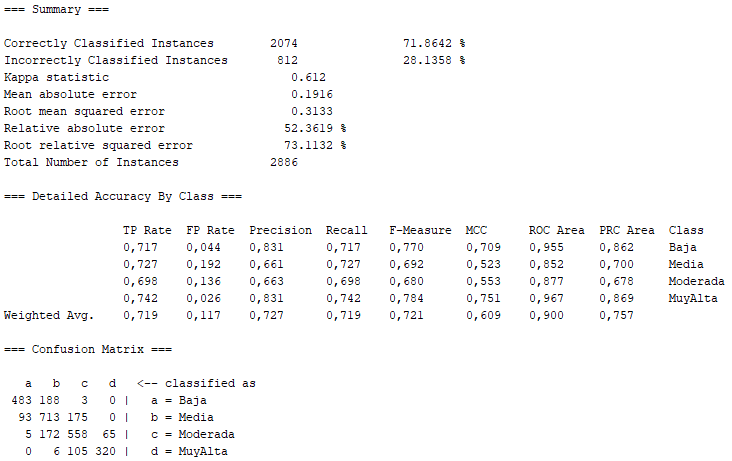
\includegraphics[scale=0.8]{clasificador-logistico-resultados-05}
    \caption{Resultados tras normalización de datos}
    \label{fig:clasificador-logistico-resultados-05}
\end{figure}

\subsection{Datos extremos}
Para la detección de valores extremos, haremos uso del filtro \code{InterquartileRange}. Este filtro añade a la base de datos un par de atributos para indicar si el patrón es un dato extremo o atípico (outlier). Según las transparencias, se consideran valores extremos aquellos que estén a más del doble del rango intercuartílico por debajo del cuartil 1 o por encima del cuartil 3. Aplicando la configuración correspondiente al filtro de Weka, podemos ver que aparecen 33 patrones con datos extremos tal como se muestra en la figura \ref{fig:valores-extremos}.
\begin{figure}[ht]
    \centering
    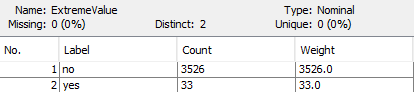
\includegraphics[scale=0.8]{valores-extremos}
    \caption{Detección de valores extremos con Weka}
    \label{fig:valores-extremos}
\end{figure}
A continuación eliminaremos los patrones con \code{ExtremeValue=yes} utilizando el filtro \code{RemoveWithValues} y posteriormente eliminaremos el atributo \code{ExtremeValues} para poder ejecutar el clasificador logístico con el conjunto de generalización. En dicha ejecución se han obtenido los valores que aparecen en la figura \ref{fig:clasificador-logistico-resultados-06}.

\begin{figure}[ht]
    \centering
    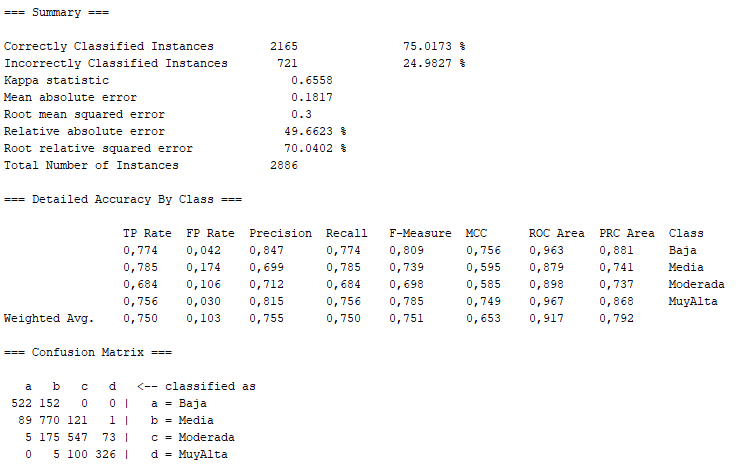
\includegraphics[scale=0.8]{clasificador-logistico-resultados-06}
    \caption{Resultados tras eliminación de valores extremos}
    \label{fig:clasificador-logistico-resultados-06}
\end{figure}

De nuevo observamos un ligero empeoramiento respecto a los resultados de partida (ver fig. \ref{fig:clasificador-logistico-resultados-04}), por lo que no parece conveniente, en este caso, eliminar los valores extremos. Esto parece lógico ya que también hay valores de este tipo en el conjunto de test, y si el modelo no los aprende, difícilmente podrá luego clasificarlos en generalización.